\section{On Real Boards: a Failure and a Fix}\label{sec:hw}

\subsection{Testbed}
We ran FOA on three ESP8266 NodeMCU boards on a phone hotspot, gossiping over ESP-NOW, with an INA226
sensor in the supply line of one board. The firmware reuses the portable C core. The feature basis is a
placeholder (not yet fitted on testbed traffic) and the keys are development keys. Two runs of about 20
minutes were logged; no attack was run on the boards.

\begin{table}[t]
\centering
\caption{Three-board testbed (medians; run in which all boards started together)}
\label{tab:hw}
\small
\begin{tabular}{@{}lr@{}}
\toprule
Cycles hearing both neighbours & 97 to 100\% \\
Update proposal / FOA step & 11.2\,ms / 1.6\,ms \\
Sign one frame / verify two & 0.60\,ms / 0.95\,ms \\
Learning cycle period & 7.77\,s \\
Board power (second run) & 365\,mW at 5.04\,V \\
Energy per cycle, whole board & 2.84\,J \\
\bottomrule
\end{tabular}
\end{table}

No extra energy for a learning cycle was detectable with the sensor sampling every 40\,ms: power in the
0.6\,s learning window was in fact $4.2\pm0.1$\,mJ \emph{below} normal running, plausibly because the
board mostly waits for frames then. About 19\,ms of computing per cycle at full board power would be
about 7\,mJ; this is an estimate. Deployment also exposed defects that simulation had not: frames were
rejected because boards boot at different times (now each sender's cycle number must only increase), and
calibration ran before the damped statistics had settled (now preceded by a warm-up).

\subsection{The collapse}
When all three boards started together, every detector's spread shrank to under 2\% of its calibrated
value within 20 minutes and false alarms reached about 90\% (Figure~\ref{fig:hw}). The board traffic is
highly repetitive. The core-only rule may shrink the spread freely while growth is gated by outer-ring
support, a one-way ratchet; identical boards agree on the shrink, and FOA applies it as common change.
In a second run, two restarted boards beside an already collapsed one levelled off near 54\%, which is
consistent with this account but does not prove it; the placeholder basis may also contribute. A
simulation of repetitive traffic with no attacker reproduces the collapse.

\begin{figure*}[t]
\centering
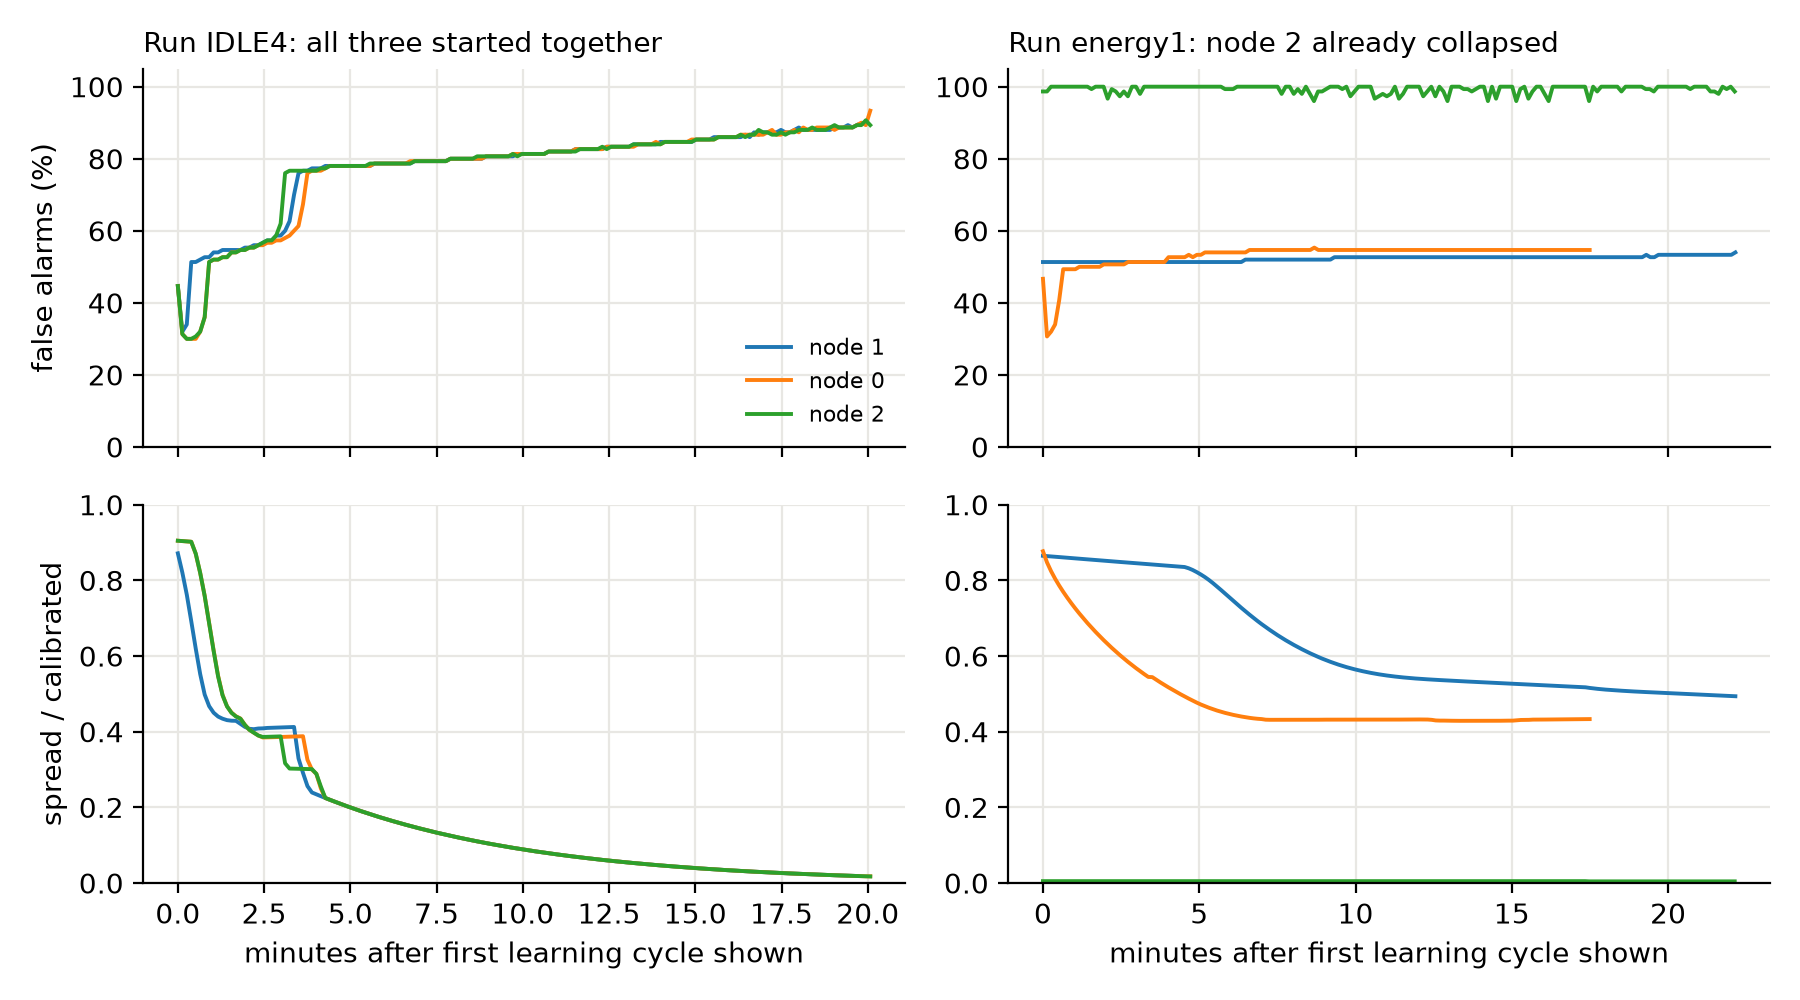
\includegraphics[width=0.85\textwidth]{figures/hardware_results.png}
\caption{The two testbed runs: false alarms and spread relative to calibration. Left: all boards started
together and collapsed. Right: one board had already collapsed; the two restarted boards levelled off.}
\label{fig:hw}
\end{figure*}

\subsection{The coverage floor}\label{sec:floor}
The fix is one rule: the spread may never shrink below its calibrated value, $s_i(t)\ge s_i^0$. It only
moves increments toward zero, so both budgets and Theorem~\ref{thm:contain} still hold (checked: no bound
violation in 1{,}710 attacked runs with the floor). We chose it on development seeds and evaluated it on
held-out seeds (Table~\ref{tab:floor}); the C core with the floor matches the reference.

\begin{table}[t]
\centering
\caption{The coverage floor on held-out seeds 2 to 11: false alarms (\%) after moderate, strong and device-only drift, and victims compromised (\%) without drift, by the boundary attacker under strong drift, and by all attackers under strong drift.}
\label{tab:floor}
\small
\setlength{\tabcolsep}{3pt}
\begin{tabular}{@{}lrrrrrr@{}}
\toprule
Rule & Mod. & Strong & Own & None & Bound. & All \\
\midrule
Single device & 18.9 & 24.6 & 20.3 & 7.4 & 63.2 & 39.2 \\
Single device + floor & 0.9 & 0.8 & 0.9 & 7.6 & 75.4 & 43.1 \\
FOA & 6.0 & 9.0 & 28.2 & 4.6 & 0.0 & 10.8 \\
\textbf{FOA + floor} & 1.4 & 2.5 & 24.6 & 4.3 & 0.0 & 9.4 \\
\bottomrule
\end{tabular}
\end{table}


On repetitive traffic (20 held-out runs) the floor cuts mean false alarms from 13.2\% to 1.5\% and the
worst run from 75\% to 5.4\%. It also changes the reading of Section~\ref{sec:eval}. \textbf{Most of
single-device adaptation's false alarms were caused by the same ratchet}: with the floor a single device
reaches \FlAutoFStrongFPR\ under strong drift, lower than FOA with the floor (\FlFOAFStrongFPR), and it
also follows its own drift far better (\FlAutoFIdioFPR\ against \FlFOAFIdioFPR). FOA's earlier
false-alarm advantage over a single device therefore does not survive. What survives, and is the reason
to use FOA, is safety under drift: with the floor in both, FOA is compromised in \FlFOAFCompStrong\ of
runs against \FlAutoFCompStrong\ for a single device, never by the boundary attacker against
\FlAutoFCompBound, and it still withstands the monoculture botnet that defeats a single device in every
run. The floored rule has not yet been run on the boards.
